\documentclass[10pt,a4paper]{article}
\usepackage[latin1]{inputenc}
\usepackage[T1]{fontenc}
\renewcommand{\rmdefault}{phv} % Arial
\renewcommand{\sfdefault}{phv} % Arial

\usepackage{calligra}

\DeclareMathAlphabet{\mathcalligra}{T1}{calligra}{m}{n}
\DeclareFontShape{T1}{calligra}{m}{n}{<->s*[2.2]callig15}{}
\newcommand{\scriptr}{\mathcalligra{r}\,}
\newcommand{\boldscriptr}{\pmb{\mathcalligra{r}}\,}
\usepackage{anysize}
\usepackage[spanish]{babel}
\usepackage{amsmath}
\usepackage{amsfonts}
\usepackage{amssymb}
\usepackage{graphicx}
\usepackage[colorlinks=true, linkcolor=red, citecolor=red, urlcolor=blue]{hyperref}
\usepackage[total={16cm,24cm},centering]{geometry}
\parskip= 5mm %espacio entre p�rrafos
\usepackage{caption} %caption personalizado
\usepackage{bm}
\usepackage{color}
\usepackage{soul}

\author{Angel Calderon}
\title{TP N�4 Introducci�n a la transformada de Fourier}
\begin{document}
\maketitle
\newpage
\tableofcontents
\newpage

\section{Definici�n de Convoluci�n}
La convoluci�n en �ptica es una herramienta esencial para modelar c�mo los sistemas �pticos transforman la luz y las im�genes, as� como para realizar an�lisis en el procesamiento de se�ales. Por ejemplo,
\begin{enumerate}
\item Holograf�a e Interferometr�a: En estos campos, la convoluci�n permite interpretar c�mo las ondas de luz se combinan para formar patrones de interferencia o im�genes hologr�ficas.
\item Microscop�a de Fluorescencia: La convoluci�n de la se�al de la muestra con la PSF del microscopio ayuda a describir la resoluci�n y calidad de la imagen capturada.
\end{enumerate}

La convoluci�n de dos funciones $h(x)$ y $g(x)$ est�n definidas como:

\begin{equation}
f(x) = (h*g)(x) = \int_{-\infty}^{\infty} h(\xi)\, g(x-\xi) d\xi
\end{equation}

\subsection{Funciones Especiales}

\begin{equation}
rect(x) =
\begin{cases} 
1 & \text{si } |x| \leq \frac{1}{2}, \\
0 & \text{si } |x| > \frac{1}{2}.
\end{cases}
\end{equation}

\section{Ejercicio 8}

\textbf{a)} La convoluc�on de $rect(\xi)$ consigo misma implica encontrar el �rea de superposici�n entre la funci�n $rect(\xi)$ y su versi�n desplazada $rect(x-\xi)$

\begin{equation}
f(x) = rect(x)*rect(x) = \int_{-\infty}^{\infty} rexct(\xi)\, rect(x-\xi) d\xi
\end{equation}

\begin{figure}[h]
\centering
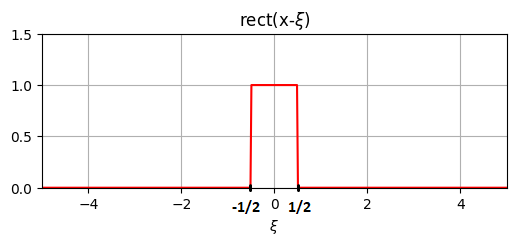
\includegraphics[scale=0.56]{rect.png}
\hfill
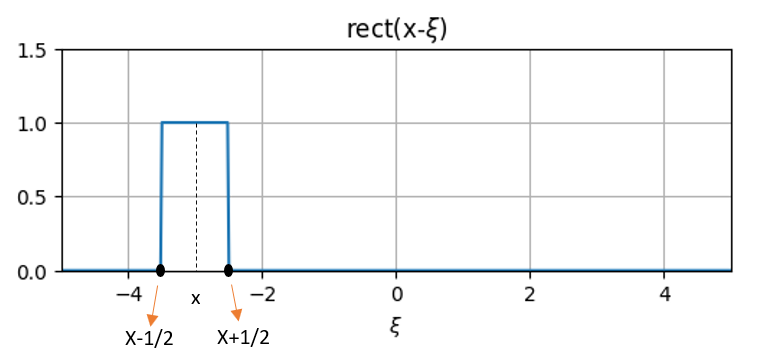
\includegraphics[scale=0.38]{rect_tras.png}
\caption{}\label{}

\end{figure}

Primero vamos a encontrar la regi�n donde el producto de las funciones no se anula.

\[rect(\xi) =
\begin{cases} 
1 & \text{si } |\xi| \leq \frac{1}{2}, \\
0 & \text{si } |\xi| > \frac{1}{2}.
\end{cases} \hspace{1cm}\Rightarrow\hspace{1cm} -\frac{1}{2}\leq\xi\leq\frac{1}{2}\]

\[rect(x-\xi) =
\begin{cases} 
1 & \text{si } |x-\xi| \leq \frac{1}{2}, \\
0 & \text{si } |x-\xi| > \frac{1}{2}.
\end{cases} \hspace{1cm}\Rightarrow\hspace{1cm} x-\frac{1}{2}\leq\xi\leq x+\frac{1}{2}\]


Nos interesa el caso donde haya intersecci�n, producto no nulo. Vamos a dividir el an�lisis en dos partes.

\begin{figure}[h!]
\centering
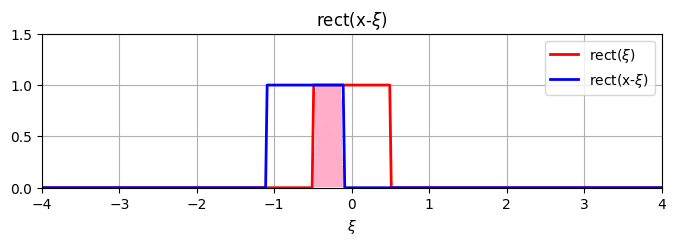
\includegraphics[scale=0.6]{rect_rect_int.png}
\caption{}\label{}
\end{figure}

\textbf{i)} $-1\leq x \leq 0$

En esta parte se integra desde lado izquierdo de $rect(\xi)$ que es $\xi=1/2$ hasta el lado derecho de $rect(x-\xi)$ que es $\xi = x+1/2$

\begin{equation}
\int_{1/2}^{x+1/2} 1 \cdot 1 d\xi = x+1
\end{equation}

\textbf{ii)} $0\leq x \leq 1$

En esta parte se integra desde lado izquierdo de $rect(x-\xi)$ que es $\xi = x-1/2$ hasta el lado derecho de $rect(\xi)$ que es $\xi = 1/2$

\begin{equation}
\int_{x-1/2}^{1/2}1 \cdot 1 d\xi = -x+1
\end{equation}

Luego, la convoluci�n queda:

\begin{equation}
f(x) = h*g=
\begin{cases}
0 & \text{si } |x|>1 \\
x+1 & \text{si } -1\leq x \leq 0 \\
-x+1 & \text{si } 0\leq x \leq 1
\end{cases}
\end{equation}

\begin{figure}[h!]
\centering
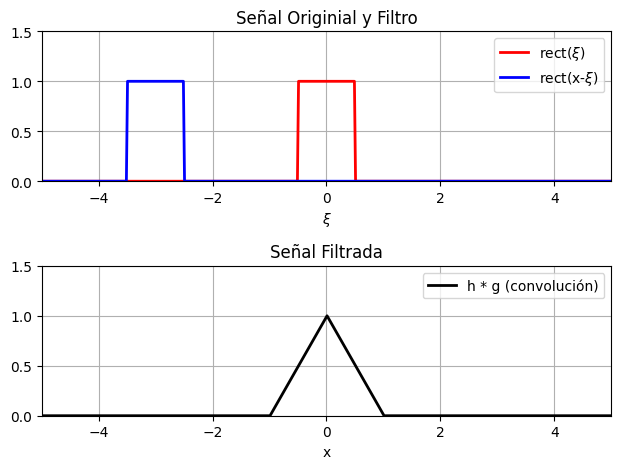
\includegraphics[scale=0.8]{rect_rect.png}
\caption{}\label{}
\end{figure}

\section{Ejercicio 7}

Una se�al $E(t) = E_0 \cos(w_0 t)$ se modula en amplitud por un pulso gaussiano $g(t) = e^{t^2/ \tau^2}$. Encuentra el espectro en el dominio de frecuencia de la se�al modulada $E_m(t) = E(t)\cdot g(t)$

B�sicamente, hay que calcular la transformada de Fourier del producto $E(t)\cdot g(t)$. Usando las propiedades de la transformada de Fourier $F$.




\end{document}